\documentclass[11pt]{article}

\usepackage{amsmath, amssymb, fancyhdr, enumitem, mathtools}
\oddsidemargin 0cm \topmargin -2cm \textwidth 16.5cm \textheight 23.5cm \parindent 0pt \parskip 0.5em

% header
\title{Parallel Algorithms for Greedy Graph Coloring - Checkpoint}
\date{April 26, 2021}
\author{Sarah Pethani (spethani) and Jeff Tan (jefftan)}

% structure
\newcommand{\question}[3]{\vspace{1em}\qb{Question #1:} #2\vspace{0.5em}\hrule\vspace{0.75em}#3\clearpage\break}
\newcommand{\qop}[2] {\newcommand{#1}{\operatorname{#2}}}
\newcommand{\qdef}[2] {\newcommand{#1}{\qtm{#2}}}


% shortcuts
\newcommand{\qC}{\mathbb{C}}
\newcommand{\qN}{\mathbb{N}}
\newcommand{\qQ}{\mathbb{Q}}
\newcommand{\qR}{\mathbb{R}}
\newcommand{\qZ}{\mathbb{Z}}
\newcommand{\qP}{\mathbb{P}}
\newcommand{\qE}{\mathbf{E}}
\newcommand{\qpow}{\mathcal{P}}
\newcommand{\qbi}{\Leftrightarrow}
\newcommand{\qimp}{\Rightarrow}
\newcommand{\qand}{\wedge}
\newcommand{\qor}{\vee}
\newcommand{\qAnd}{\bigwedge}
\newcommand{\qOr}{\bigvee}
\newcommand{\qint}{\cap}
\newcommand{\quni}{\cup}
\newcommand{\qInt}{\bigcap}
\newcommand{\qUni}{\bigcup}
\newcommand{\qemp}{\varnothing}
\newcommand{\qsub}{\subseteq}
\newcommand{\qsups}{\supseteq}
\newcommand{\qsm}{\setminus}
\newcommand{\qtilde}{\sim}
\newcommand{\qt}{\textrm}
\newcommand{\qtm}{\mathrm}
\newcommand{\qb}{\textbf}
\newcommand{\qi}{\textit}
\newcommand{\qbb}{\mathbf}
\newcommand{\qu}{\underline}
\newcommand{\qof}{\circ}
\newcommand{\qrest}{\restriction}
\newcommand{\qblank}{\sqcup}
\newcommand{\qfrom}{\leftarrow}
\newcommand{\qdx}{\frac d{dx}}
\newcommand{\qpar}[2] {\frac{\partial #1}{\partial #2}}
\newcommand{\qov}{\overline}
\newcommand{\qch}[2] {{#1\choose #2}}
\newcommand{\qinv}{\phantom}
\newcommand{\qd}{\displaystyle}
\newcommand{\qdt}{\textstyle}
\newcommand{\qpr}[1] {\qprob\qpc{#1}}
\newcommand{\qexp}[1] {\qE\qpb{#1}}
\newcommand{\qvar}[1] {\qVar\qp{#1}}
\newcommand{\qcov}[1] {\qCov\qp{#1}}
\qop{\qdim}{dim}
\qop{\qspan}{span}
\qop{\qgcd}{gcd}
\qop{\qdet}{det}
\qop{\qsign}{sgn}
\qop{\qproj}{proj}
\qop{\qinf}{inf}
\qop{\qsup}{sup}
\qop{\qmeas}{meas}
\qop{\qVar}{\qbb{Var}}
\qop{\qCov}{\qbb{Cov}}
\qop{\qprob}{\qbb P}
\qop{\qnotice}{notice}
\qop{\qnegl}{negl}
\newcommand{\qfl}[1] {\left\lfloor #1 \right\rfloor}
\newcommand{\qceil}[1] {\left\lceil #1 \right\rceil}
\newcommand{\qlen}[1] {\left\lVert #1 \right\rVert}
\newcommand{\qabs}[1] {\left| #1 \right|}
\newcommand{\qp}[1] {\left( #1 \right)}
\newcommand{\qpb}[1] {\left[ #1 \right]}
\newcommand{\qpc}[1] {\left\{ #1 \right\}}
\newcommand{\qpa}[1] {\left\langle #1 \right\rangle}
\newcommand{\qmatrix}[1] {\qpb{\begin{matrix} #1 \end{matrix}}}
\newcommand{\qlist}[1] {\begin{enumerate} #1 \end{enumerate}}
\newcommand{\qlista}[1] {\begin{enumerate}[label=(\alph*)] #1 \end{enumerate}}
\newcommand{\qlistn}[1] {\begin{enumerate}[label=\arabic*)] #1 \end{enumerate}}
\newcommand{\qlistb}[1] {\begin{itemize}[label=\textbullet~] #1 \end{itemize}}
\newcommand{\qlistr}[1] {\begin{enumerate}[label=(\roman*)] #1 \end{enumerate}}
\newcommand{\qlistA}[1] {\begin{enumerate}[label=\Alph*.] #1 \end{enumerate}}
\newcommand{\qlistR}[1] {\begin{enumerate}[label=\Roman*.] #1 \end{enumerate}}
\newcommand{\qtable}[2] {\begin{displaymath}\begin{array}{#1} #2 \end{array}\end{displaymath}}
\newcommand{\qalign}[1] {\begin{align*} #1 \end{align*}}
\newcommand{\qalignn}[1] {\begin{align}\setcounter{equation}{0} #1 \end{align}}
\newcommand{\qcenter}[1] {\begin{center} #1 \end{center}}
\newcommand{\qquote}[1] {\begin{quote} #1 \end{quote}}
\newcommand{\qcases}[1] {\begin{cases*} #1 \end{cases*}}
\renewcommand{\mod} {\operatorname{mod}}
\renewcommand{\inf} {\infty}
\renewcommand{\hat} {\widehat}
\renewcommand{\tilde} {\widetilde}

\begin{document}                        

\thispagestyle{plain}
\maketitle

\section{Summary}
We are going to implement different parallel algorithms for greedy graph coloring in OpenMP and possibly CUDA. We will analyze/compare their performance, speedup, and solution quality (e.g. does one algorithm use less colors than another).

\section{Progress}
Currently, we have implemented a baseline greedy sequential algorithm for graph coloring, as well as the Jones-Plassman (JP) and Gebremedhin-Manne (GM) algorithms which run in parallel using OpenMP. These algorithms produce valid colorings on sparse graphs, dense graphs, and other randomly generated graphs, and we are currently working on speeding them up. We have tested these algorithms on a variety of graphs to verify correctness.\\

Specifically, to test our graph coloring algorithms, we have written a script to generate random graphs with an arbitrary number of vertices according to the Erdos-Renyi model, where each edge is included with some fixed probability p, independently of all other edges. Depending on the value of p, Erdos-Renyi is able to produce dense graphs, fully connected sparse graphs, as well as forests with many separate connected components. In addition to using Erdos-Renyi, we may also consider testing our algorithms on existing graph algorithm benchmarks.\\

For input to the algorithms, we save each graph as a file where the first line contains the total number of vertices, and the remaining lines each encode an edge in the graph between two vertices. The vertices are 0-indexed, where no vertex may be higher than the number of vertices - 1. All of the algorithms rely on a graph class which we created, which parses the input file and creates an adjacency list representation of the graph in order to provide constant-time neighbor access.\\

\section{Goals and Deliverables}
We currently have correct implementations of the JP and GM algorithms in OpenMP, and our main goal is to optimize their performance to achieve good speedup on Gates and Latedays. Our progress is in line with the schedule that we provided in the proposal, and as such, we may not have time to achieve our stretch goal of implementing these graph algorithms in CUDA, as implementing graph algorithms on GPUs is significantly more challenging.

Our planned schedule for the remaining weeks is as follows:
\qlistb{
	\item Thu 04/29
	\qlistb{
		\item Sarah: Profile JP implementation and try to speed up parallel implementation; try to eliminate memory contention
		\item Jeff: Profile GM implementation and try to speed up parallel implementation
	}
	\item Mon 05/03
	\qlistb{
		\item Sarah: Try different ways of parallelizing work, in addition to parallelizing the loops suggested in the pseudocode for JP algorithm
		\item Jeff: Try different ways of parallelizing work, in addition to parallelizing the loops suggested in the pseudocode for GM algorithm
	}
	\item Thu 05/06
	\qlistb{
		\item Sarah: Look into memory access pattern of JP to try and eliminate false sharing and improve locality
		\item Jeff: Look into alternative graph representations that improve the memory access pattern of GM, and try to improve locality on large graphs
		\item Both: Create a representative set of test graphs (sparse, dense, fully connected, not connected, etc.) to test speedup and execution time
	}
	\item Mon 05/10
	\qlistb{
		\item Sarah: Generate final performance data for JP algorithm v. baseline sequential
		Jeff: Generate final performance data for GM algorithm v. baseline sequential
		\item Both: Start preparing the project report and presentation
	}
	\item Thu 05/13
	\qlistb{
		\item Both: Finalize and submit project report and presentation
	}
}

\section{Plan to Present}
We plan to present the performance, speedup, and solution quality of both parallel algorithms on varying types of graphs, as well as qualitative conclusions about the tradeoffs between the algorithms. To determine these metrics, we plan to generate a representative set of benchmarks to test our algorithms on, and we will present charts and tables illustrating the speedup, execution time, and number of colors used for each algorithm.

\section{Preliminary Results}
$$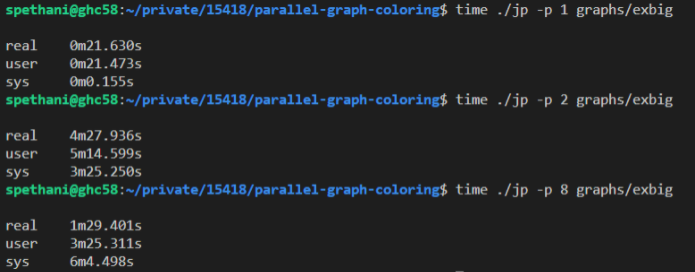
\includegraphics[scale=0.75]{checkpoint_jp.png}$$
For JP, the algorithm becomes much slower when introducing parallelism/using OpenMP. This can be seen from the jump in time from using 1 processor to using 2 processors instead. There is speedup when increasing the number of processors when comparing it to the 2 processor time, but the execution time is laughable compared to the sequential execution. This will have to be looked into further, to understand why introducing OpenMP creates such a large slowdown. These preliminary results are on a dense graph with 10k vertices. 

$$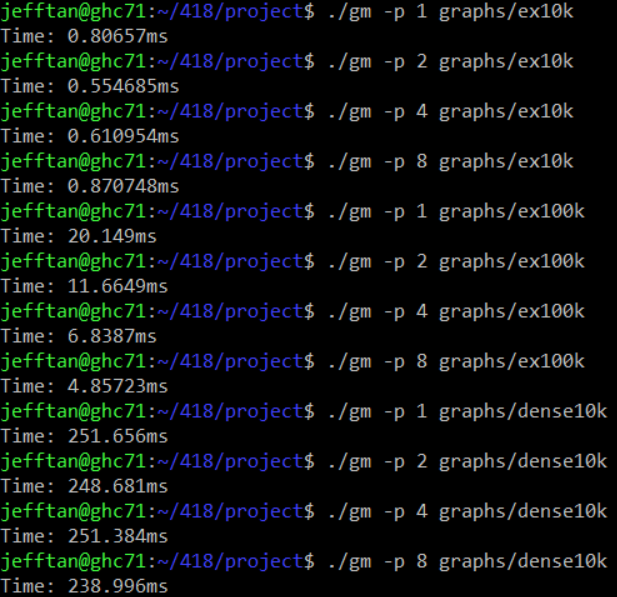
\includegraphics[scale=0.5]{checkpoint_gm.png}$$
For GM, our speedup differs greatly based on the type of input graph we are providing. For small graphs like ex10k (a sparse graph with 10k vertices), using more processors makes the runtime slightly longer, likely because the overhead of introducing parallelism is not worth the very slight benefits that parallelism would provide. For medium-sized graphs like ex100k (a sparse graph with 100k vertices), using more processors provides some speedup. However, for very large graphs like dense10k (a fully connected graph with 10k vertices), using more processors yields no speedup over a single processor, likely because the graphs are too big to fit into memory at this point, so the main bottleneck of the code is memory access. We plan to perform additional experiments to determine how our code performs on different types of graphs.

\section{Current Challenges}
Currently, our parallel implementations of the JP and GM algorithms do not perform faster than the sequential baseline when parallelized.\\

In the JP algorithm, this could be due to the critical section around the addition of vertices to the independent set which we are coloring, but it could also be a result of the graphs we are testing on not being large enough. This is a plausible issue, as the loops which are parallelized over all vertices do not show significant speedup over their sequential counterparts, which will most likely change as we increase the number of vertices significantly.\\

In the GM algorithm, this could be due to our parallel work distribution method. Currently, within each iteration, we determine which colors are allowed for each vertex in parallel, and we update the remaining worklist in parallel. However, this results in a lot of synchronization between threads, as the algorithm constantly has to perform in parallel and synchronize back together. The GM algorithm also performs poorly when operating on large graphs because it keeps separate data structures for each thread, reducing locality by making the working set too large to fit in cache. We hope to improve these issues by reconsidering our work distribution between threads and possibly adjusting our graph representation to better provide spatial locality.\\

If we still encounter issues with the parallelization of these algorithms, we will reach out to our TA mentor.\\

\end{document}